\documentclass[10pt]{beamer}

% ------------------------------------------------------------------------
% Preambulo personalizado
% ------------------------------------------------------------------------
\usetheme[progressbar=frametitle]{metropolis}
\usepackage{appendixnumberbeamer}
\usepackage{fancyvrb}
\usepackage{booktabs}
\usepackage[scale=2]{ccicons}
\usepackage{pgfplots}
\usepgfplotslibrary{dateplot}
\usepackage{type1cm}
\usepackage{lettrine}
\usepackage{ragged2e}
\usepackage{xspace}
\newcommand{\themename}{\textbf{\textsc{metropolis}}\xspace}
\usepackage{graphicx} % Allows including images
\usepackage{booktabs} % Allows the use of \toprule, \midrule and \bottomrule in tables
\usepackage[utf8]{inputenc} %solucion del problema de los acentos.
\usepackage{xcolor}
\definecolor{LightGray}{gray}{0.9}

\usepackage{minted}
\usemintedstyle{tango}
\newcommand{\mypyfile}[1]{\inputminted[linenos=true, fontsize=\footnotesize, frame=lines, framesep=5\fboxrule,framerule=1pt]{python}{#1}}

\setminted[python]{breaklines,frame=lines,framesep=2mm,baselinestretch=1.2,bgcolor=LightGray,linenos, fontsize=\footnotesize} % obeytabs=true, tabsize=2, showtabs=true}

%%%%%%%%%%%%%%%%%%%%%%%%%%%%%%%%%%%%%%%%%%%%%%%%%%%%%%%%%%%%%%%%%%%%%%%%%%%%%%%%%%%%%%
\setbeamercolor{progress bar}{fg=blue!50!black,bg=white!50!black}
\setbeamercolor{title separator}{fg=red!50!black,bg=white!50!black}
\setbeamercolor{frametitle}{fg=white!80!black,bg=red!50!black}
\title[PCFI161]{Programaci\'on para F\'isica y Astronom\'ia}
\subtitle{Departamento de Física.}

\newcommand{\myfront}{
\author[PCFI161]{Corodinadora: C Loyola \\ Profesoras/es C Loyola / C Femenías / Y Navarrete / C Ruiz}
\institute[UNAB]{Universidad Andrés Bello}
\date{Primer Semestre 2025}
}

\titlegraphic{%
  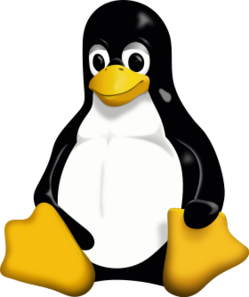
\includegraphics[width=.08\textwidth]{logo-tux.png}\hfill
  
\includegraphics[width=.3\textwidth]{logo-unab.png}\hfill
  
\includegraphics[width=.08\textwidth]{logo-python.png}
}

\makeatletter
\setbeamertemplate{title page}{
  \begin{minipage}[b][\paperheight]{\textwidth}
    \vfill%
    \ifx\inserttitle\@empty\else\usebeamertemplate*{title}\fi
    \ifx\insertsubtitle\@empty\else\usebeamertemplate*{subtitle}\fi
    \usebeamertemplate*{title separator}
    \ifx\beamer@shortauthor\@empty\else\usebeamertemplate*{author}\fi
    \ifx\insertdate\@empty\else\usebeamertemplate*{date}\fi
    \ifx\insertinstitute\@empty\else\usebeamertemplate*{institute}\fi
    \vfill
    \ifx\inserttitlegraphic\@empty\else\inserttitlegraphic\fi
    \vspace*{1cm}
  \end{minipage}
}
\makeatother


\makeatletter
\setlength{\metropolis@titleseparator@linewidth}{2pt}
\setlength{\metropolis@progressonsectionpage@linewidth}{2pt}
\setlength{\metropolis@progressinheadfoot@linewidth}{2pt}
\makeatother


\title{Semana 12 – Sesión 1 (Sesión 23): Estadística descriptiva con NumPy, Pandas y Matplotlib}
\author{PCFI161 – Programación para Física y Astronomía}
\date{19 mayo 2025}

\begin{document}

% ------------------------------------------------------------------------
% Portada
% ------------------------------------------------------------------------
\myfront{}
\begin{frame}
  \titlepage
\end{frame}

% ------------------------------------------------------------------------
% Tabla de contenidos
% ------------------------------------------------------------------------
\begin{frame}
  \frametitle{Resumen – Semana 12, Sesión 1 (Sesión 23)}
  \tableofcontents
\end{frame}

\metroset{block=fill}

% --------------------------------------------------------------------------------
\section{Introducción y Repaso}
% --------------------------------------------------------------------------------
\begin{frame}{Contexto y Repaso}
  \begin{itemize}
    \item Hasta la Semana 10 trabajamos con:
      \begin{itemize}
        \item \textbf{NumPy}: arrays, álgebra lineal, aleatoriedad.
        \item \textbf{Matplotlib}: subplots, histogramas, 3D.
      \end{itemize}
    \item Hoy iniciamos la \textbf{unidad de Estadística}:
      \begin{itemize}
        \item Medidas descriptivas (media, mediana, varianza).
        \item Uso de \texttt{pandas} para tablas de datos.
        \item Visualización: histogramas, boxplots, violin plots.
      \end{itemize}
    \item \alert{Tarea V} se publicará al final de la segunda sesión.
  \end{itemize}
\end{frame}

% --------------------------------------------------------------------------------
\section{Objetivos de la Sesión}
% --------------------------------------------------------------------------------
\begin{frame}{Objetivos}
  \begin{itemize}
    \item Comprender \textbf{estadística descriptiva} con \texttt{NumPy}.
    \item Manejar \textbf{DataFrames} de \texttt{pandas} para resumen rápido.
    \item Generar \textbf{gráficos estadísticos} en Matplotlib.
    \item Preparar bases para la \textbf{Tarea V} (análisis de datos reales).
  \end{itemize}
\end{frame}

% --------------------------------------------------------------------------------
\section{Medidas Descriptivas con NumPy}
% --------------------------------------------------------------------------------
\begin{frame}[fragile]{NumPy: estadísticas básicas}
\begin{minted}{python}
import numpy as np
data = np.random.normal(loc=0, scale=1, size=1_000)

print("Media :", data.mean())
print("Mediana :", np.median(data))
print("Desvío estándar :", data.std(ddof=1))
print("Percentiles 25/75 :", np.percentile(data, [25, 75]))
\end{minted}
\begin{itemize}
  \item \texttt{ddof=1} usa varianza muestral (\(n-1\)).
  \item \texttt{np.percentile} devuelve los cuantiles solicitados.
\end{itemize}
\end{frame}

% --------------------------------------------------------------------------------
\section{Resumen con pandas}
% --------------------------------------------------------------------------------
\begin{frame}[fragile]{pandas: \texttt{describe()} y más}
\begin{minted}{python}
import pandas as pd

df = pd.DataFrame({"x": data})
print(df.describe())
\end{minted}
\begin{itemize}
  \item \texttt{describe()} produce conteo, media, std, min, max y cuartiles.
  \item \(\rightarrow\) Ideal para inspección rápida de datasets.
\end{itemize}
\end{frame}

% --------------------------------------------------------------------------------
\section{Visualización de Datos}
% --------------------------------------------------------------------------------
\begin{frame}[fragile]{Histogramas y Boxplots}
\begin{minted}{python}
import matplotlib.pyplot as plt

fig, axs = plt.subplots(1, 2, figsize=(8,4))

axs[0].hist(df["x"], bins=30, alpha=0.8)
axs[0].set_title("Histograma")

axs[1].boxplot(df["x"], vert=False, patch_artist=True)
axs[1].set_title("Boxplot")

plt.tight_layout(); plt.show()
\end{minted}
\begin{itemize}
  \item El boxplot muestra mediana, cuartiles y outliers.
  \item \texttt{patch\_artist=True} permite colorear la caja.
\end{itemize}
\end{frame}

% --------------------------------------------------------------------------------
\section{Ejercicios Prácticos}
% --------------------------------------------------------------------------------
\begin{frame}{Ejercicio 1: Estadística de Alturas}
  \begin{block}{Enunciado}
    \begin{itemize}
      \item Cargar el archivo \texttt{alturas.csv} (columna \emph{height\_cm}).
      \item Usar \textbf{NumPy} y \textbf{pandas} para calcular: media, mediana, desvío y cuartiles.
      \item Graficar histograma y boxplot en la misma figura.
      \item Comentar si los datos muestran \emph{sesgo} o \emph{asimetría}.
    \end{itemize}
  \end{block}
\end{frame}

\begin{frame}{Ejercicio 2: Correlación Masa-Altura (opcional)}
  \begin{block}{Pasos}
    \begin{enumerate}
      \item Cargar \texttt{masas\_alturas.csv} con columnas \texttt{mass\_kg}, \texttt{height\_cm}.
      \item Calcular coeficiente de correlación \(\rho\) con \texttt{np.corrcoef}.
      \item Graficar scatter y ajustar recta (\texttt{np.polyfit}).
    \end{enumerate}
  \end{block}
\end{frame}

% --------------------------------------------------------------------------------
\section{Cierre}
% --------------------------------------------------------------------------------
\begin{frame}{Próxima Sesión}
  \begin{itemize}
    \item \textbf{Sesión 24 (en dos días)}: Taller evaluado + publicación de \textbf{Tarea V}.
    \item Traer notebook listo y datasets descargados.
  \end{itemize}
\end{frame}

\end{document}
